\documentclass[12pt]{beamer}

\usetheme{Oxygen}
\setbeamertemplate{navigation symbols}{}
\setbeamertemplate{footline}{}

\setbeamercovered{transparent}

\usepackage[utf8]{inputenc}
\usepackage[spanish]{babel}
\usepackage{verbatim}
\usepackage{lgrind}
\usepackage{listings}
\usepackage{beamertexpower}
\usepackage{amsmath}
\usepackage{array}

\pdfinfo
{
  /Title       (QTestLib)
  /Creator     (Kile)
  /Subject     (Testeo de aplicaciones y librerias)
  /Author      (Rafael Fernandez Lopez)
}

\title{KDE 4}
\author{Rafael Fernández López, Aleix Pol i Gonzàlez}
\institute{}
\date{Marzo 2008}

\lstset{
  basicstyle=\ttfamily,
  showstringspaces=false,
  language=
}

\begin{document}

\begin{frame}
	\titlepage
	\frametitle{Aditel iParty X}
	\framesubtitle{ereslibre@kde.org, aleixpol@gmail.com}
	\begin{center}
	
\includegraphics[width=2.2cm]{imatges/kde.png}
	\end{center}
\end{frame}

\section*{}
\begin{frame}
  \frametitle{Contenidos}
  \tableofcontents
\end{frame}


\section{Introducción}
%-------------------------------------------------------------------
\subsection{Comunidad KDE}
	\begin{frame}
		\frametitle{Nosotros}
		\begin {itemize}
			\item 11 años
			\item +1600 cuentas svn
			\item 65 idiomas
			\item Millones de usuarios alrededor del mundo
		\end {itemize}
	\end{frame}

%-------------------------------------------------------------------
\section{Tecnologías}
\subsection{Belleza}

\begin {frame}
\frametitle{Belleza}
\begin{center}
	
\includegraphics[width=150px]{imatges/beauty.png}
\end{center}
\end {frame}

\begin{frame}
\frametitle{Plasma}
\begin{center}
	
\includegraphics[width=150px]{imatges/plasma.png}
\end{center}
\end{frame}
\begin{frame}
\frametitle{Oxygen}
\begin{center}
	
\includegraphics[width=150px]{imatges/oxygen.png}
\end{center}
\end {frame}
%-------------------------------------------------------------------
\subsection{Portabilidad}
\begin {frame}
	\frametitle{Portabilidad}
	\begin{center}
	
\includegraphics[width=150px]{imatges/portability.png}
	\end{center}
\end {frame}

\begin{frame}
	\frametitle{ Multiplataforma }

	\center 
\includegraphics[width=250px]{imatges/plataformas.png}

\end{frame}

%-------------------------------------------------------------------
\subsection{Funcionalidad}
\begin {frame}
\frametitle{Funcionalidad}

\begin{center}
	
\includegraphics[width=100px]{imatges/function.png}
\end{center}
\end {frame}


\begin {frame}
\frametitle{Solid}
\begin{center}

\includegraphics[width=150px]{imatges/solid.png}
\end{center}
\end {frame}

\begin {frame}
\frametitle{Phonon}
\begin{center}

\includegraphics[width=200px]{imatges/phonon.png}
\end{center}
\end {frame}

\begin {frame}
\frametitle{Sonnet}
\begin{center}
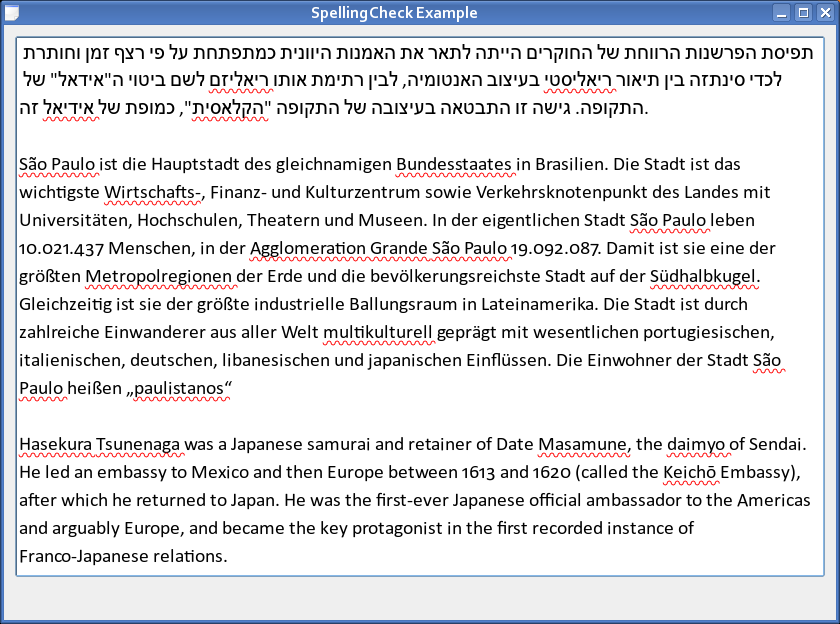
\includegraphics[width=200px]{imatges/sonnet.png}
\end{center}
\end {frame}

\begin {frame}
\frametitle{Akonadi}
\begin{center}
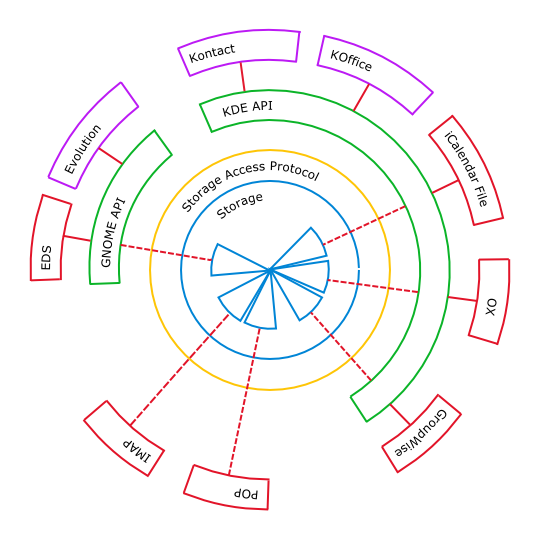
\includegraphics[height=200px]{imatges/akonadi.png}
\end{center}
\end {frame}

\begin {frame}
\frametitle{ThreadWeaver}
\begin{center}
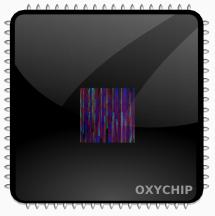
\includegraphics[width=100px]{imatges/threadweaver.png}
\end{center}
\end {frame}

\begin {frame}
\frametitle{Strigi + Nepomuk}
\begin{center}

\includegraphics[width=75px]{imatges/strigi.png}

\includegraphics[width=150px]{imatges/nepomuk.png}
\end{center}
\end {frame}

\begin {frame}
\frametitle{Raptor}
\begin{center}

\includegraphics[width=200px]{imatges/raptor.png}
\end{center}
\end {frame}

\begin {frame}
\frametitle{Kross}
\begin{center}
\huge { Kross }
\end{center}
\end {frame}
%-------------------------------------------------------------------

%-------------------------------------------------------------------
\section {Conclusiones}
\begin{frame}
	\frametitle{Recordatorio}
	\begin{alertblock}{Alerta!!!}
		KDE4 no es KDE 4.0!!
	\end{alertblock}
	Esto sólo es el principio!
\end{frame}
\begin{frame}
	\frametitle{Colabora!}
	
	\begin{itemize}
	\item Traduciendo
	\item Dibujando
	\item Documentando
	\item Mejorando la web
	\item Dando soporte a los usuarios
	\item OpenUsability
	\item Programando
	\end{itemize}
	
	\begin{flushright}
		
\includegraphics[width=70px]{imatges/konqi.png}
	\end{flushright}
\end{frame}
\begin{frame}
\frametitle{Preguntes}
\huge { Alguna pregunta? }
\begin{flushright}
	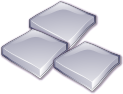
\includegraphics[width=100px]{imatges/blocs.png}
\end{flushright}
\end{frame}
%-------------------------------------------------------------------

\end{document}
